\documentclass[10pt]{beamer} % For a presentation we need to use the document class "beamer"
% Here we can also define the font size (10pt)

% This template uses the Metropolis theme by Matthias Vogelgesang (https://www.overleaf.com/latex/templates/metropolis-beamer-theme/qzyvdhrntfmr) and is meant to present an easily accessible template for everyone who wants to set-up a quick-and-easy presentation

%%%%%%%%%%%%%%%%%%%%%%%%%%%%%%%%%%%%%%%%%%%%%%%%%%%%%%%%%%%%%%%%%
% This file contains all style information and loads additional packages that are necessary for the generation of the presentation
%%%%%%%%%%%%%%%%%%%%%%%%%%%%%%%%%%%%%%%%%%%%%%%%%%%%%%%%%%%%%%%%%

%%%%%%%%%%%%%%%%%%%%%%%%%%%%%%%%%%%%%%%%%%%%%%%%%%%%%%%%%%%%%%%%%
% Load the theme

% Use the Metropolis theme
\usetheme[progressbar=frametitle]{metropolis} % Adds a progress bar to the frametitle
% The template for the Metropolis theme can be accessed here: https://de.overleaf.com/latex/templates/metropolis-beamer-theme/qzyvdhrntfmr

% Change the width of the progress bar to make it more visible (Code taken from here: https://github.com/matze/mtheme/issues/237)
\makeatletter
\setlength{\metropolis@titleseparator@linewidth}{0.5pt} % Title page
\setlength{\metropolis@progressonsectionpage@linewidth}{1.5pt} % Progress bar on section page
\setlength{\metropolis@progressinheadfoot@linewidth}{1.5pt} % Progress bar in header
\makeatother

% Change the color of the progress bar to match it with the logo
% First we need to define the colors
\definecolor{darkblue}{RGB}{32,61,86}
\definecolor{blue}{RGB}{62, 129, 171}
% And then we set the color for the progressbar
\setbeamercolor{progress bar}{fg=blue,
  bg=alerted text.fg!70!black!20}
% "fg" presents the already presented part and "bg" the part to come (we use the standard color for "bg")

% We also need to adjust the color for the alert text
\setbeamercolor{alerted text}{fg=blue}

% And the alerted box
\setbeamercolor{alerted box}{fg=blue}

% Change frame title color
\setbeamercolor{frametitle}{bg=darkblue}

% Change title slide so that the line is a bit thicker (comment if you want the original title page)
% The code was inspired by this code: https://tex.stackexchange.com/questions/512146/beamer-theme-customizing-title-page
\setbeamertemplate{title page}{
{%
% Add the logo
\begin{flushright}
    \inserttitlegraphic
    \end{flushright}
    }
% Add the title and the subtitle
 {%
    \usebeamercolor[fg]{title}
    \usebeamerfont{title}
        \inserttitle\\
        \medskip
        \textnormal{\large\insertsubtitle}
    }
    \par\smallskip
% Define the line and the line width
{%
    \color{blue!50!blue}
        \rule{\linewidth}{1.1pt}
    }
    \par\smallskip
% Add the author
    {%
    \usebeamercolor[fg]{author}
    \usebeamerfont{author}
        \insertauthor
    }\par\smallskip
% Add the date
    {%
    \usebeamercolor[fg]{date}
    \usebeamerfont{date}
        \insertdate
    }\par
% Add the institute
    {%
    \usebeamercolor[fg]{institute}
    \usebeamerfont{institute}
        \insertinstitute
    }
}


%%%%%%%%%%%%%%%%%%%%%%%%%%%%%%%%%%%%%%%%%%%%%%%%%%%%%%%%%%%%%%%%%
% Load relevant packages
\usepackage{appendixnumberbeamer}

\usepackage{booktabs}
\usepackage[scale=2]{ccicons}

\usepackage{pgfplots}
\usepgfplotslibrary{dateplot}

\usepackage{xspace}
\newcommand{\themename}{\textbf{\textsc{metropolis}}\xspace}

\usepackage{hyperref}
\pdfstringdefDisableCommands{%
  \let\enspace\empty  % this causes the warning for \kern
  \let\noindent\empty % this causes the warning for \indent
}

% Package for citation
\usepackage[sort]{natbib} % We use natbib in this example

% For citing with natbib, you may want to use this reference sheet: 
% http://merkel.texture.rocks/Latex/natbib.php

\bibliographystyle{apsr} % We use the APSR style % Loads required packages from the separate file 


%%%%%%%%%%%%%%%%%%%%%%%%%%%%%%%%%%%%%%%%%%%%%%%%%%%%%%%%%%%%%%%%%
% Add title information
\title{Sleep State Prediction Using Accelerometry Data\space } % Adds the title of the presentation
\subtitle{Francisco Jose de Caldas District University} % Comment if you do not need it
\date{\footnotesize \today} % Adds the date (default: today
\author[Authors]{Authors \\ Juan Carlos Quintero Rubiano \\ Code: 20232020172
                \\ Juan Nicolas Diaz Salamanca \\ Code: 20232020059 
                \\ Juan Felipe Wilches Gomez \\ Code: 20231020137}
\institute{Francisco Jose de Caldas District University} % Adds the author's institute/university
\titlegraphic{\hfill
\includegraphics[height=2cm]{figures/logo.png}} % Adds a logo 

%%%%%%%%%%%%%%%%%%%%%%%%%%%%%%%%%%%%%%%%%%%%%%%%%%%%%%%%%%%%%%%%%
% Begin the document
\begin{document}

\maketitle % Adds the title

%%%%%%%%%%%%%%%%%%%%%%%%%%%%%%%%%%%%%%%%%%%%%%%%%%%%%%%%%%%%%%%%%
% Add an agenda
\begin{frame}[plain]{Outline} % "Plain" omits the page number
%    \tableofcontents[hideallsubsections] % Adds table of content and hides all subsections
   \tableofcontents % Adds table of content 
\end{frame}
\section{Introduction}
\begin{frame}{Introduction} % Add frame title
 % We use the environment "columns" to generate a slide with an image and a text side-by-side. "Columns" is provided by beamer
 % And this command defines the width of the text
\normalsize \centering \textbf{How does it study sleep?}
 \begin{itemize}
     \item \footnotesize Sleep is a fundamental complex biological process composed of \textbf{several distinct states} which interruptions  or unbalanced on this process may come with important  \textbf{physical and mental health issues}, affecting millions worldwide and are linked to chronic diseases.
     \item \footnotesize Traditionally sleep had been studied using Polysomnography (PSG) a technology that captures detailed physiological signals. However, \textbf{PSG requires specialized facilities,
     trained technicians, and sophisticated instrumentation}.
     \item Recent advances in wearable technology have enabled the use of accelerometers as a non-invasive, low-cost alternative for sleep state prediction. These sensors, embedded in consumer devices like smartwatches and fitness trackers, measure body movement to infer sleep and wake state:
 \end{itemize}
        
\end{frame}

\section{Sleep System Approach}

\begin{frame}{Sleep system approach} % Add frame title
 % This command defines the width of the image
          \begin{figure}
              \centering
             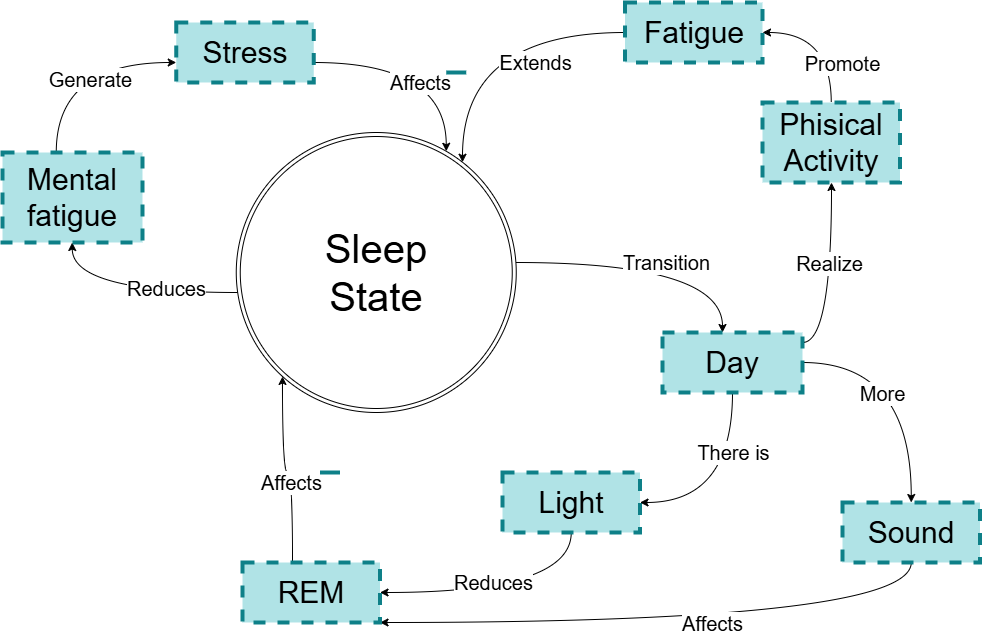
\includegraphics[width=0.8\textwidth]{figures/simulation.png} % The scale reduced the size of the image
             \caption{Sleep system diagram} % We add a caption again
             \end{figure}
% And this command defines the width of the text
 
\end{frame}
\begin{frame}{Sleep system approach} % Add frame title
 % This command defines the width of the image
          \begin{figure}
              \centering
             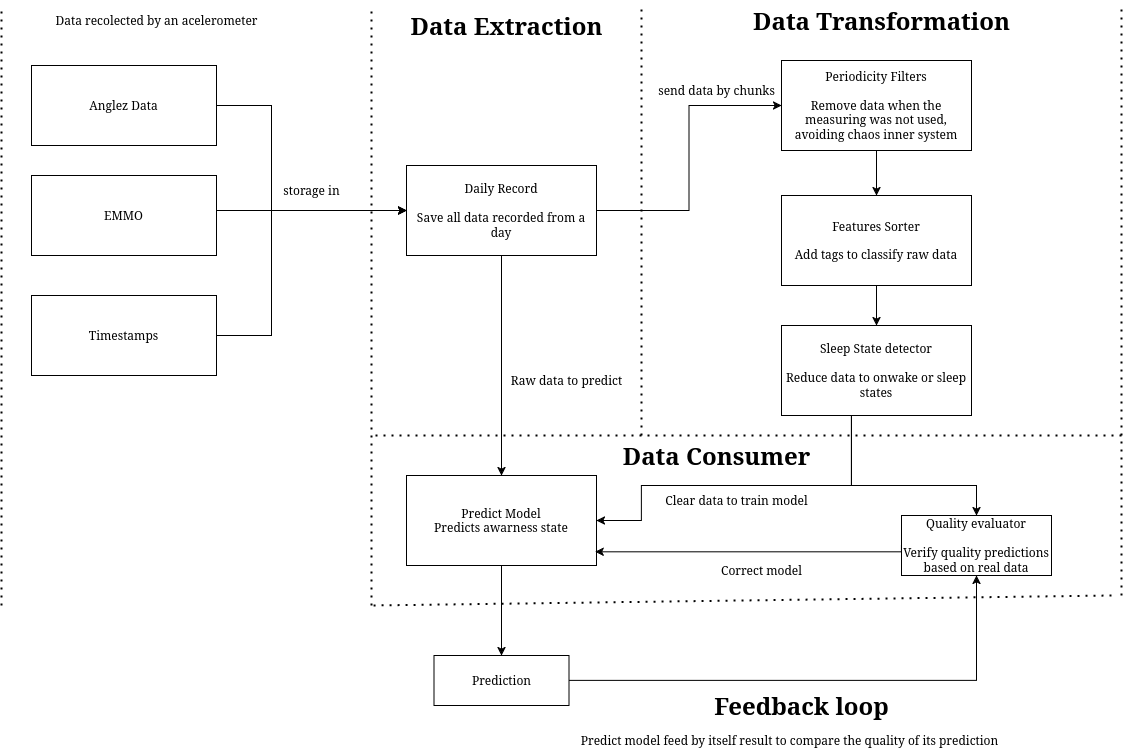
\includegraphics[width=0.95\textwidth]{figures/system.png} % The scale reduced the size of the image
             \caption{Architecture diagram} % We add a caption again
             \end{figure}
% And this command defines the width of the text
 
\end{frame}
\begin{frame}{Sleep system approach: Data Extraction  } % Add frame title
 % This command defines the width of the image
 \begin{itemize}
    \item \footnotesize ENMO: Euclidean Norm Minus One, a measure of physical activity.
    \item \footnotesize Anglez: Angle of the wrist, which can indicate the position of the wrist.
    \item \footnotesize Step: step identifier.
    \item \footnotesize Timestamp: Measurement time.
\footnotesize ENMO and Anglez are normalized
\end{itemize}
          \begin{figure}
              \centering
             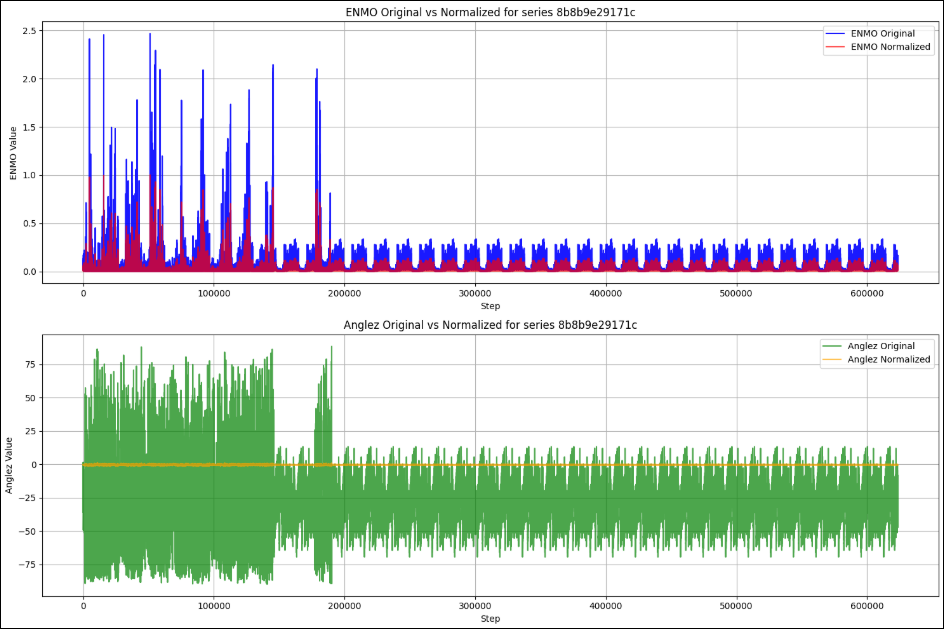
\includegraphics[width=0.6\textwidth]{figures/data_normalizate.png} % The scale reduced the size of the image
             \caption{Data normalized} % We add a caption again
             \end{figure}
% And this command defines the width of the text

\end{frame}

\begin{frame}{Sleep system approach: Data Transformation  } % Add frame title
 % This command defines the width of the image
\begin{itemize}
    \item \footnotesize Sadeh algorithm Activity-based sleep-wake identification: an empirical test of methodological issues
    \item \footnotesize Cole-Kripke Algorithm automatic sleep/wake identification from wrist activity
    \item \footnotesize OPAL Algorithm for sleep/wake classification using activity and posture.
	This version uses a logistic regression-inspired approach to combine features
\end{itemize}
    \begin{figure}[htb]
    \centering
    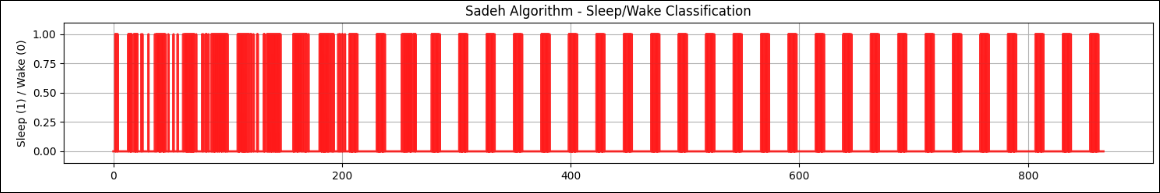
\includegraphics[width=0.8\textwidth]{figures/sadeh_result.png}
    \end{figure}
    \begin{figure}[htb]
    \centering
    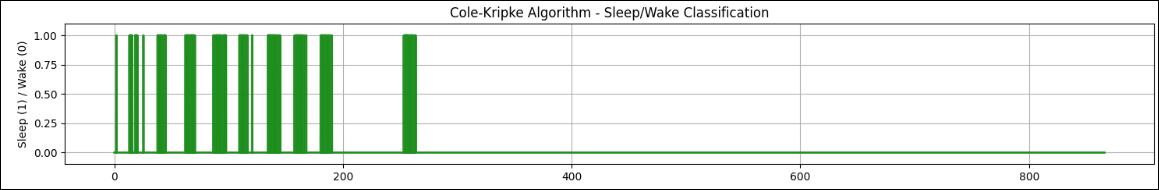
\includegraphics[width=0.8\textwidth]{figures/Cole_result.png}
    \end{figure}
    \begin{figure}[htb]
    \centering
    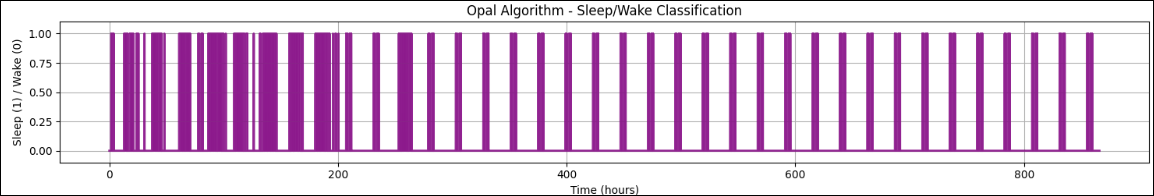
\includegraphics[width=0.8\textwidth]{figures/Opal_result.png}
    \end{figure}
% And this command defines the width of the text

\end{frame}

\begin{frame}{Sleep system approach: Data Consumers } % Add frame title
 % This command defines the width of the image
 \begin{itemize}
    \item \footnotesize The data from every algorithm is divided by 180 in order to get 15 minutes intervals to, which 10 minutes are used to train the model and 5 minutes
    to predice and comparate to analyze the model precision. 
\end{itemize}
          \begin{figure}
            
             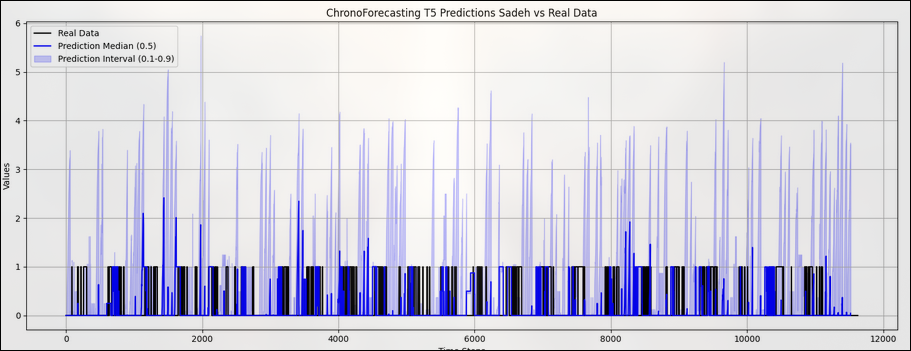
\includegraphics[width=0.8\textwidth]{figures/sadehvsReal.png} % The scale reduced the size of the image
             \end{figure}
\end{frame}

\begin{frame}{Quality metrics}
        \begin{figure}
      
        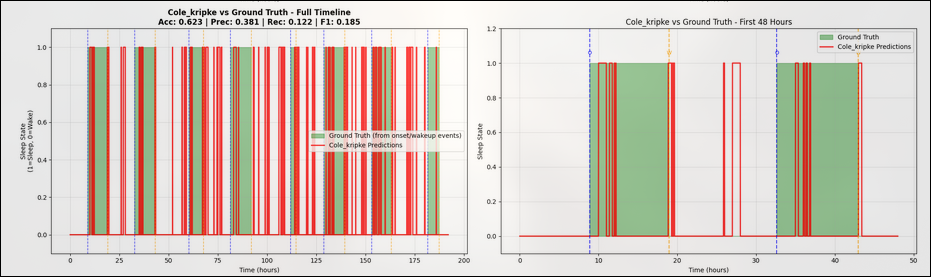
\includegraphics[width=0.9\textwidth]{figures/colevsGReal.png} % The scale reduced the size of the image
        \end{figure}
        \begin{figure}
        \centering
        \includegraphics[width=0.9\textwidth]{figures/opalvsGReal.png} % The scale reduced the size of the image
        \end{figure}
\end{frame}

\section{Results}

\begin{frame}{Algorithm Performance Comparison - Code Execution Example}
\begin{itemize}
  \item \footnotesize This example demonstrates the actual performance metrics obtained from our compiled code implementation
  \item \footnotesize Performance evaluation is based on ground truth comparison from sleep event annotations
\end{itemize}

\begin{table}[h]
\centering
\footnotesize
\begin{tabular}{|l|c|c|c|c|}
\hline
\textbf{Algorithm} & \textbf{Accuracy} & \textbf{Precision} & \textbf{Recall} & \textbf{F1-Score} \\
\hline
Sadeh & 0.7040 & 0.1579 & 0.1390 & 0.1479 \\
Cole-Kripke & 0.7043 & 0.1784 & 0.1667 & 0.1723 \\
OPAL & \textcolor{red}{\textbf{0.5902}} & \textcolor{red}{\textbf{0.2105}} & \textcolor{red}{\textbf{0.4429}} & \textcolor{red}{\textbf{0.2853}} \\
\hline
\end{tabular}
\end{table}

\begin{itemize}
  \item \footnotesize \textcolor{red}{\textbf{Best performing algorithm: OPAL (F1-Score: 0.2853)}}
  \item \footnotesize OPAL demonstrates superior balance between precision and recall
  \item \footnotesize Higher recall indicates better sleep event detection capability
\end{itemize}
\end{frame}

\begin{frame}{OPAL Algorithm - Detailed Event Analysis}
\footnotesize \textbf{Real-time Event Detection Performance (Code Execution Sample):}

\begin{table}[h]
\centering
\tiny
\begin{tabular}{|l|c|c|c|c|c|c|}
\hline
\textbf{Event} & \textbf{Step} & \textbf{Epoch} & \textbf{Predicted} & \textbf{Ground Truth} & \textbf{Expected} & \textbf{Match} \\
\hline
onset & 25548 & 2129 & 1 & 1 & 1 & \textcolor{green}{\textbf{$\checkmark$}} \\
wakeup & 31932 & 2661 & 1 & 1 & 0 & \textcolor{red}{\textbf{$\times$}} \\
onset & 43488 & 3624 & 1 & 1 & 1 & \textcolor{green}{\textbf{$\checkmark$}} \\
wakeup & 49224 & 4102 & 1 & 1 & 0 & \textcolor{red}{\textbf{$\times$}} \\
onset & 59580 & 4965 & 0 & 1 & 1 & \textcolor{red}{\textbf{$\times$}} \\
wakeup & 67272 & 5606 & 0 & 1 & 0 & \textcolor{green}{\textbf{$\checkmark$}} \\
onset & 77640 & 6470 & 1 & 1 & 1 & \textcolor{green}{\textbf{$\checkmark$}} \\
wakeup & 83844 & 6987 & 0 & 1 & 0 & \textcolor{green}{\textbf{$\checkmark$}} \\
\hline
\end{tabular}
\end{table}

\begin{itemize}
  \item \footnotesize \textbf{Event Detection Rate:} 62.5\% correct predictions (5/8 events)
  \item \footnotesize \textbf{Sleep Onset Detection:} 75\% accuracy (3/4 onsets correctly detected)
  \item \footnotesize \textbf{Wake Detection:} 50\% accuracy (2/4 wakeups correctly detected)
  \item \footnotesize This demonstrates the algorithm's preference for sleep state detection over wake transitions
\end{itemize}
\end{frame}

\begin{frame}{Implementation Notes}
\begin{itemize}
  \item \footnotesize \textbf{Important:} These results represent a specific execution example of our compiled code
  \item \footnotesize The performance metrics may vary depending on the dataset and individual sleep patterns
  \item \footnotesize This example illustrates the methodology rather than following the sequential diagram flow
  \item \footnotesize OPAL's superior F1-score indicates better overall balance for clinical applications requiring sleep event detection
  \item \footnotesize The modular architecture allows for independent algorithm optimization and real-time performance evaluation
\end{itemize}
\end{frame}

\section{Conclusions}

\begin{frame}{Conclusions}
\begin{itemize}
  \item The system is linear and deterministic, with modular components depending on the correct functioning of previous stages and a feedback loop that reinitializes processing to resolve errors and enhance reliability.

  \item  A built-in validation module ensures error tolerance by detecting anomalies and reprocessing data from the point of failure to maintain result integrity.

  \item A data filtering mechanism restricts invalid or irrelevant input under certain conditions to ensure only valid data is processed.

\end{itemize}
\end{frame}
\begin{frame}{Conclusions}
\begin{itemize}
      \item  The architecture follows a modular and structured pipeline: raw data is processed (normalization, filtering, smoothing), features are extracted, and relevant data is sent to a deep learning model for event detection.

      \item  Detected events go through validation and are then formatted and exported; this modular flow supports scalability, reuse, and adaptability to changing data or models.

     \item  Components can be tested and upgraded independently, improving system robustness, fault tolerance, and resilience to data variability and randomness.

     \item  Limitations include sensitivity to chaotic inputs (e.g., sleep disturbances from medication), environmental randomness, and sensor failures, requiring continuous adaptation and relying on advanced validation and pre-trained LLMs to reduce false outcomes.
\end{itemize}

\end{frame}

%%%%%%%%%%%%%%%%%%%%%%%%%%%%%%%%%%%%%%%%%%%%%%%%%%%%%%%%%%%%%%%%%

\end{document} % End the document here
